\documentclass[twoside]{article}
\usepackage[a4paper]{geometry}
\geometry{verbose,tmargin=2.5cm,bmargin=2cm,lmargin=2cm,rmargin=2cm}
\usepackage{fancyhdr}
\pagestyle{fancy}

% nastavení pisma a~češtiny
\usepackage{lmodern}
\usepackage[T1]{fontenc}
\usepackage[utf8]{inputenc}
\usepackage[czech]{babel}

% odkazy
\usepackage{url}

\usepackage{float}
% vícesloupcové tabulky
\usepackage{multirow}
\usepackage{amssymb}
\usepackage{gensymb}
\usepackage{bbold}
\usepackage{amsmath}
\usepackage{mathtools}
\usepackage{commath}

% vnořené popisky obrázků
\usepackage{subcaption}

% automatická konverze EPS 
\usepackage{graphicx} 
\usepackage{epstopdf}
\epstopdfsetup{update}

\graphicspath{{./images}}

% odkazy a~záložky
\usepackage[unicode=true, bookmarks=true,bookmarksnumbered=true,
bookmarksopen=false, breaklinks=false,pdfborder={0 0 0},
pdfpagemode=UseNone,backref=false,colorlinks=true] {hyperref}

% Poznámky při překladu
\usepackage{xkeyval}	% Inline todonotes
\usepackage[textsize = footnotesize]{todonotes}
\presetkeys{todonotes}{inline}{}

%https://tex.stackexchange.com/questions/2783/bold-calligraphic-typeface
\DeclareMathAlphabet\mathbfcal{OMS}{cmsy}{b}{n}

% Zacni sekci slovem ukol
\renewcommand{\thesection}{Úkol \arabic{section}}
% enumerate zacina s pismenem
\renewcommand{\theenumi}{\alph{enumi}}

% smaz aktualni page layout
\fancyhf{}
% zahlavi
\usepackage{titling}
\fancyhf[HC]{\thetitle}
\fancyhf[HLE,HRO]{\theauthor}
\fancyhf[HRE,HLO]{\today}
 %zapati
\fancyhf[FLE,FRO]{\thepage}

% údaje o autorovi
\title{Automatické řízení: DÚ 8 -- Stavové metody}
\author{Vojtěch Michal}
\date{\today}

\begin{document}

\maketitle

\section{Model HIV - AIDS}
Nemoc AIDS dosud nedokážeme s jistotou plně vyléčit ani nedokážeme z těla pacienta úplně odstranit virus
HIV. Stále lépe ale dokážeme pomocí léků udržet počet částic viru v těle pacienta na nízké úrovni a tím
bránit vzniku nemoci AIDS.

Stavový model nákazy krevních buněk CD4+T, které virus HIV napadá, je po linearizaci v ekvilibriu
odpovídajícím bezpříznakovému pacientu dán rovnicemi

\begin{equation}
	\begin{split}
		\begin{bmatrix}
			\dot{T} \\
			\dot{T^{*}} \\
			\dot{\nu}
		\end{bmatrix} &= \underbrace{\begin{bmatrix}
			-0.04167 & 0 & -0.0058 \\
			0.0217 & -0.24 & 0.0058 \\
			0 & 100 & -2.4
		\end{bmatrix}}_{\mathbf{A}} \underbrace{\begin{bmatrix}
		T \\
		T^{*} \\
		\nu
	\end{bmatrix}}_{ \vec{x}} + \underbrace{\begin{bmatrix}
		5.2 \\
		-5.2 \\
		0
	\end{bmatrix}}_{\mathbf{B}} u \\
	y &= \underbrace{\begin{bmatrix}
		0 & 0 & 1
	\end{bmatrix}}_{\mathbf{C}} \begin{bmatrix}
		T \\
		T^{*} \\
		\nu
	\end{bmatrix}
\end{split}
\label{eq:zadani}
\end{equation}
Stavové veličiny $T$, $T^{*}$, $\nu$ jsou po řadě počet zdravých buněk, počet infikovaných buněk a počet volných
částic viru v krevním řečišti pacienta. Model zahrnuje léčbu pacienta pomocí léků RTI (inhibitory reverzní
transkriptázy) a tak je vstupem relativní dávkování RTI  $u \in [0,1]$ v rozsahu nulová až plná dávka. Výstupem
je počet volných částic viru.

Navrhněte řízení pomocí stavové zpětné vazby se specifikacemi: $e_{ss,step} = 0$, $OS\% = 10\%$, $T_s = 100~\text{dnů}$.
Přitom volte variantu zajišťující nulovou ustálenou odchylku robustně, tedy integrální řízení. \\
\\
\textbf{Řešení:}
V rovnici \eqref{eq:zadani} jsou pojmenovány matice stavového modelu pomocí standardního značení $\mathbf{A}$, $\mathbf{B}$, $\mathbf{C}$.
Vektor stavů $T$, $T^{*}$ a $\nu$, označíme $\vec{x}$.
Nejprve se zaměřím na splnění požadavků na dynamiku systému zadaných pomocí maximálního overshootu a doby ustálení.

Samotná soustava je zřejmě třetího řádu a má přenos
\begin{equation}
	G(s) = \mathbf{C} (sI - \mathbf{A})^{-1} \mathbf{B} =  \frac{-520(s+0.0200)}{(s+2.6433)(s+0.0192+0.0658i)(s+0.0192-0.0658i)}.
\end{equation}

\subsection{Požadavky na dynamiku}
Pomocí dvou požadavků se nám podaří umístit dva póly uzavřené smyčky, systém je ale zřejmě třetího řádu. Prozatím budu dynamiku 
navrhovat pro dominantní dvojici pólů -- tedy jakoby systém řádu 2 -- a třetím pólem zkusím později pokrátit nějakou nulu, nebo jej 
dám dostatečně daleko vlevo od dominantní dvojice. Zadaný maximální překmit CL nám určuje minimální damping ratio
\begin{equation}
	\zeta = \frac{- \text{ln}(OS\%/100)}{\sqrt{\pi^2 + \text{ln}^2(OS\%/100)}} = 0.5912.
\end{equation}
Předpokládejme, že ustálení má nastat na dvě procenta.
S pomocí relativního tlumení a požadovaného času ustálení lze vypočíst přirozenou frekvenci
\begin{equation}
	\omega_n =  -\frac{\text{ln}(0.02 \cdot \frac{\sqrt{1-\zeta^2}}{\zeta})}{\zeta \cdot T_s}
	 = 0.0609~\text{rad} \cdot \text{den}^{-1} = 7.0509 \cdot 10^{-7} \text{rad} \cdot \text{s}^{-1}.
\end{equation}
Protože pro dominantní póly platí $Re(p) = \omega_n \zeta$ a $Im(p) = \omega_n \sqrt{1-\zeta^2}$, nalézají se v bodech 
\begin{equation}
	p_{1,2} = (-4.1682 \pm 5.6870i) \cdot 10^{-7}.
\end{equation}
Jejich vliv proto velmi výrazně (o pět dekád) dominuje nad vlivem nuly v bodě $z = -0.02$ a použití vzorců pro 
systém řádu 2 nezanáší do návrhu podstatnou chybu.
Nulu $z$ pokrátíme posledním zbylým pólem. Cílem návrhu je dát uzavřené ZV smyčce charakteristický polynom
\begin{equation}
	c(s) = (s^2 + 2\omega_n \zeta s + \omega_n^2) (s+0.02).
\end{equation}
Před hledáním regulátoru jsem ověřil, že $\text{rank}(\mathcal{C}) = \text{rank}(\mathbf{A})$ a systém je tedy úplně řiditelný.
Pro nalezení regulátoru použiji Ackermannův vzorec
\begin{equation}
	K = \begin{bmatrix}
		0 & 0 & 1
	\end{bmatrix} \mathcal{C}^{-1}  c(\mathbf{A}) = \begin{bmatrix}
		-0.0042 & 0.5077 & -0.0122
	\end{bmatrix},
	\label{eq:acker}
\end{equation}
v němž figuruje inverze matice řiditelnosti $\mathcal{C}$ a $c(\mathbf{A})$ je dosazení matice 
systému do nového žádaného char. polynomu $c(s)$.

Uzavřením stavové zpětné vazby s regulátorem $K$ vzniká nový systém s maticí 
\begin{equation}
	\mathbf{A}_{new} = \mathbf{A} - \mathbf{B}K = \begin{bmatrix}
		-0.02 &   -2.64 &    0.0576 \\
		3.4694 \cdot 10^{-18}  &   2.4  &  -0.0576   \\
			 0  & 100  &  -2.4
	\end{bmatrix}.
\end{equation}
Na obrázku \ref{fig:wrong_gain} je výsledek simulace odezvy uzavřené smyčky na jednotkový skok. Již na první pohled je patrné,
že matice systému je extrémně blízko signulárnosti (prvek $\mathbf{A}_{new_{21}}$ je již na hranici numerických chyb)
a bude tak potřeba se systémem dále hýbat.

\begin{figure}[htbp]
	\centering
	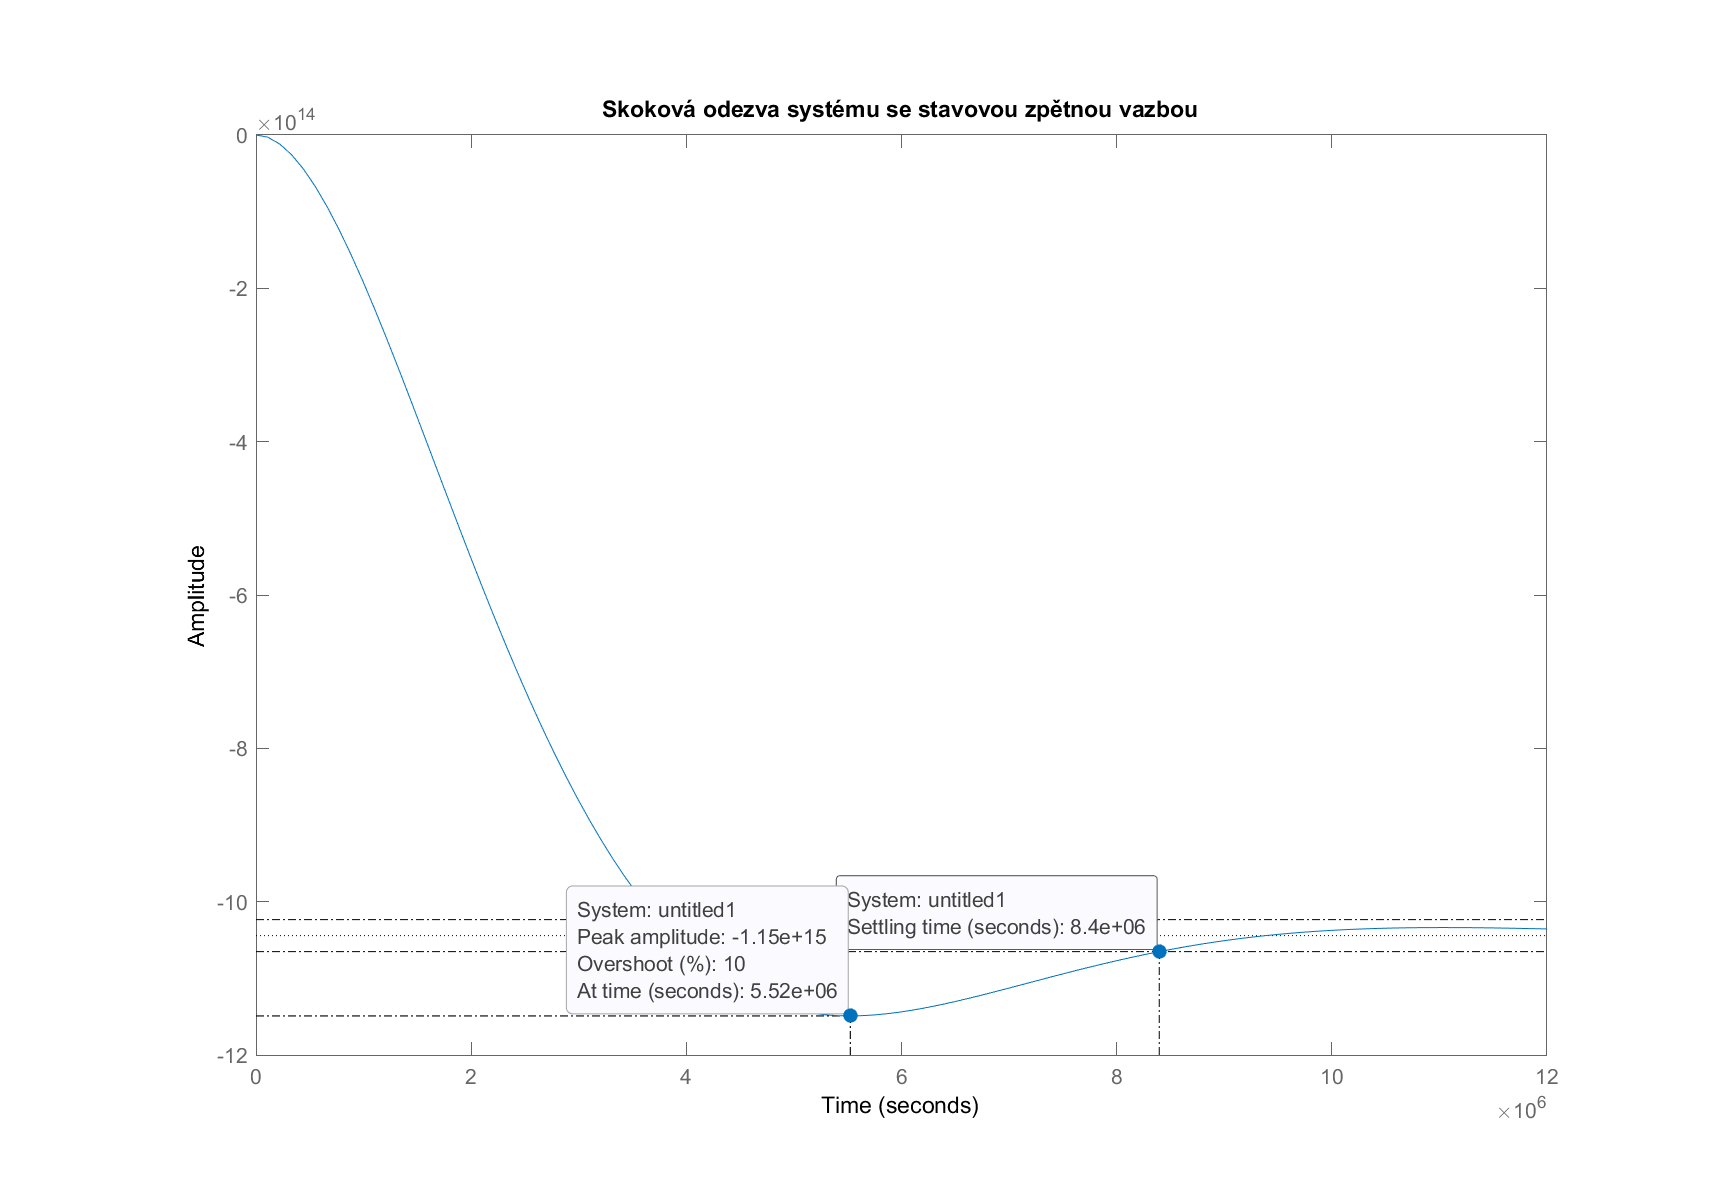
\includegraphics[width=\linewidth]{skokova_odezva.eps}
	\caption{Simulace odezvy soustavy po zavedení stavové zpětné vazby}
	\label{fig:wrong_gain}
\end{figure}
Překmit odezvy skutečně nepřesahuje 10\% a ustálení nastane po $100 \times 24 \times 3600 = 8640000$ sekundách.
Požadavky na dynamiku systému jsou splněny, jenom ta amplituda v řádu $10^{14}$ není v pořádku.

\subsection{Nastavení ustálené odchylky}
Uzavřená smyčka stavové zpětné vazby není schopna asymptoticky sledovat jednotkový skok. Použití feedforwardu pro nastavení
statického zesílení není přípustné s ohledem na robustnost, je tak nezbytné použít integrální řízení.
Vzniká systém řádu 4 se stavovým modelem
\begin{equation}
	\begin{split}
		\begin{bmatrix}
			\dot{\vec{x}} \\ \dot{x_I}
		\end{bmatrix} &= \underbrace{ \begin{bmatrix}
			\mathbf{A} & 0 \\
			-\mathbf{C} & 0
		\end{bmatrix}}_{\mathbf{A}_{big}} \underbrace{ \begin{bmatrix}
			\vec{x} \\ x_I
		\end{bmatrix}}_{\vec{x_{big}}} + \underbrace{\begin{bmatrix}
			\mathbf{B} \\ 0
		\end{bmatrix}}_{\mathbf{B}_{big}} r \\
		y &= \underbrace{\begin{bmatrix}
			\mathbf{C} & 0
		\end{bmatrix}}_{\mathbf{C}_{new}} \begin{bmatrix}
			\vec{x} \\ x_I
		\end{bmatrix}.
	\end{split}
\end{equation}

Nasazením Ackermannova vzorce podobně jako v \eqref{eq:acker} pro něj nalezneme regulátor
\begin{equation}
	K_{final} = \begin{bmatrix}
		K & \mid & K_I
	\end{bmatrix} = \begin{bmatrix}
		-0.0042 &  -18.7231 &   0.4493 & \mid &  9.5607 \cdot 10^{-14}
	\end{bmatrix}.
\end{equation}

Zavedením zpětné vazby kolem regulátoru získáme nový systém s modelem
\begin{equation}
	\begin{split}
		\mathbf{A}_{final} &= \begin{bmatrix}
			\mathbf{A}-\mathbf{B}K & -\mathbf{B}K_I \\
			-\mathbf{C} & 0
		\end{bmatrix} \\
		\mathbf{B}_{final} &= \begin{bmatrix}
			\vec{0} \\ 1
		\end{bmatrix} \\
\mathbf{C}_{final} &= \begin{bmatrix}
	\mathbf{C} & 0
\end{bmatrix},
	\end{split}
\end{equation}
jehož odezva na jednotkový skok je vykreslena na obrázku \ref{fig:good_gain}.
\begin{figure}[htbp]
	\centering
	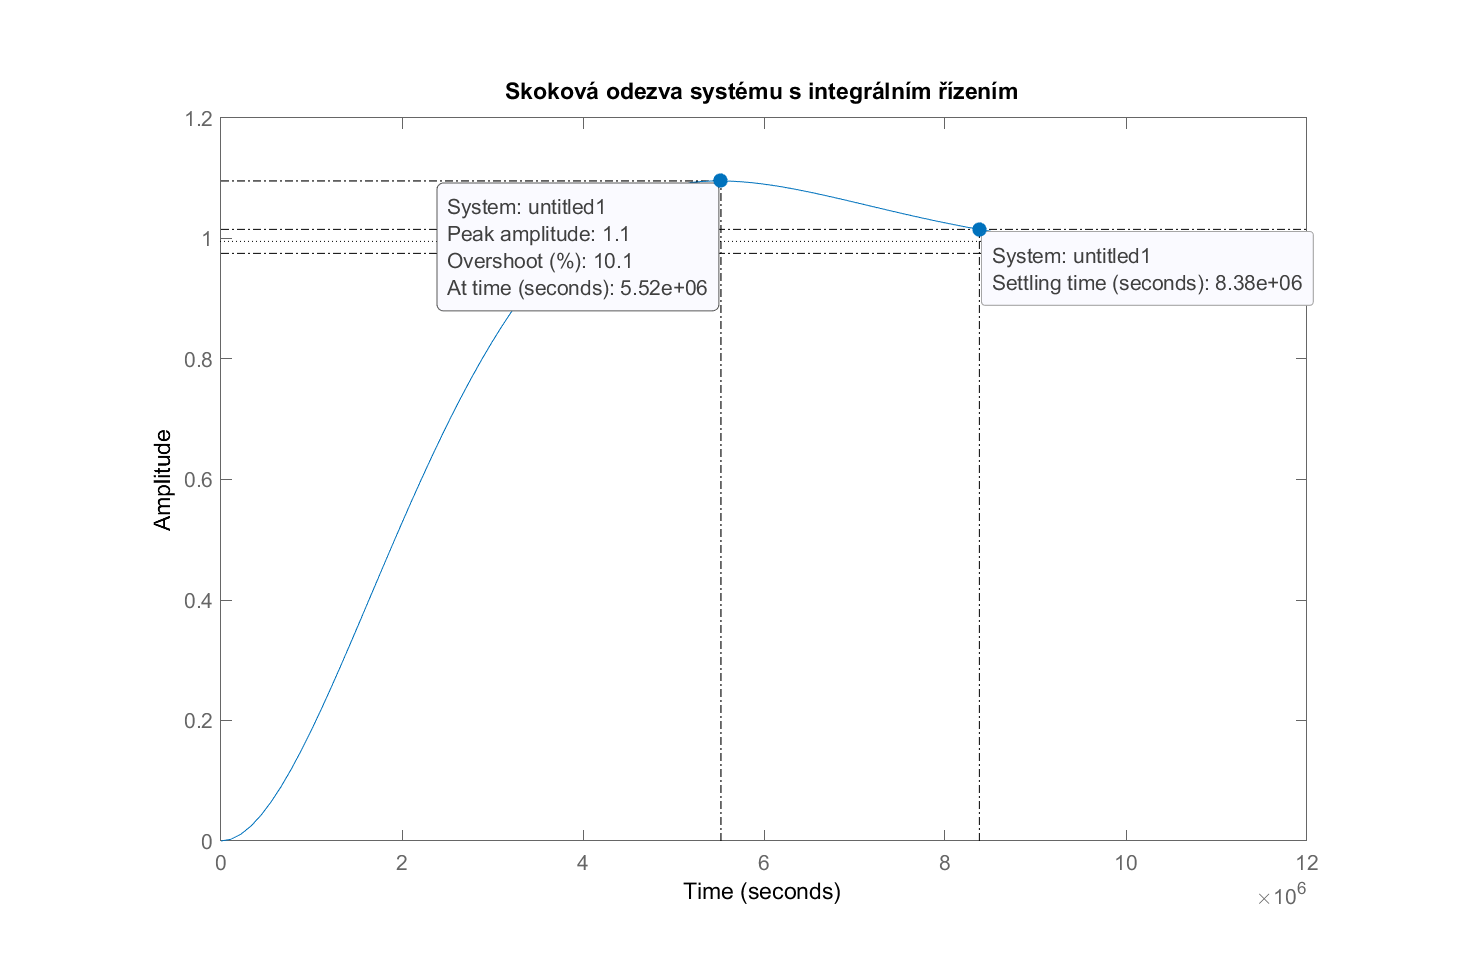
\includegraphics[width=\linewidth]{skokova_po_integraci.eps}
	\caption{Simulace odezvy soustavy po zavedení integrálního řízení}
	\label{fig:good_gain}
\end{figure}

Simulace potvrzuje dostatečné splnění stanovených požadavků na dynamiku systému a na nulovou ustálenou odchylku
odezvy na jednotkový skok. Vlivem numerických chyb během výpočtů (aritmetika s čísly o deset a víc řádů od sebe)
a dále chyby zaokrouhlování je peak overshoot o desetinu procenta vyšší, než povoleno. Tohoto nedostatku se dá
snadno zbavit například provedením výpočtu pro nižší povolený overshoot. Protože se jedná o lékařskou aplikaci a je v sázce
lidský život, rovněž by šlo relaxovat požadavek na stodenní ustálení a tím ještě více snížit overshoot použitím pozvolnějšího
časového průběhu (celkově tak zpomalit systém).


\end{document}

